\documentclass[12pt,a4paper]{article} 

\usepackage[T1]{fontenc}
\usepackage[utf8]{inputenc} 
\usepackage{amsmath, graphicx, enumerate, tabularx}
\usepackage[polish]{babel}
% asmath - math; graphicx - images; enumerate - lists
\graphicspath{ {./images/} }

\pagenumbering{gobble}
\begin{document}
\title{{
  \begin{center}
    
\includegraphics[width=8cm]{wsiz}
  \end{center}
  \vspace{1.3cm}

  \LARGE Technologie sieciowe CCNA

  \LARGE Projekt sieci internetowej - dokumentacja}}

\author{{\Large Aleksander Ordyczyński, w65557}}
\date{}
\maketitle

\newpage
\section{Opis zadania}
Zadanie polega na przydzieleniu adresacji sieci komputerowej a następnie wykonaniu prostego projektu w programie Cisco Packet Tracer.
\subsection{Adresacja}
Adres klasy B - 17.5.0.0/16 został podzielony na następujące sieci:\\
Sieć LAN A - 70 hostów\\
Sieć LAN B – 50 hostów\\
Sieć LAN C – 270 hostów\\
Sieć LAN D – 550 hostów\\
Sieć LAN E – 2 hosty\\

%  \begin{table}[]
    \begin{tabular}{|c|c|c|c|c|}
      \hline
      sieć & adres sieci &  zakres hostów  & adres broadcast & maska \\
      \hline
      A & 17.5.20.0/25 & 17.5.20.1 - 17.5.20.126  & 17.5.20.127  & 255.255.255.128  \\
      B & 17.5.30.0/26 & 17.5.30.1 - 17.5.30.62   & 17.5.30.63 & 255.255.255.192 \\
      C & 17.5.10.0/23 & 17.5.10.1 - 17.5.11.254  & 17.5.10.255 & 255.255.254.0 \\
      D & 17.5.0.0/22 & 17.5.0.1 - 17.5.3.254  & 17.5.20.255 & 255.255.252.0 \\
      E & 17.5.40.0/30 & 17.5.40.1 - 17.5.40.2   & 17.5.20.3 &  255.255.255.252 \\
      \hline
    \end{tabular}

\subsection{Packet Tracer}
1. Budowa sieci według schematu w programie Packet Tracer. \\
2. Ustawienia routerów:

a) Ustawienie adresów na interfejsach.

b) Ustawienie servera DHCP routerom.

c) Ustawienie routingu statycznego.
\begin{center}
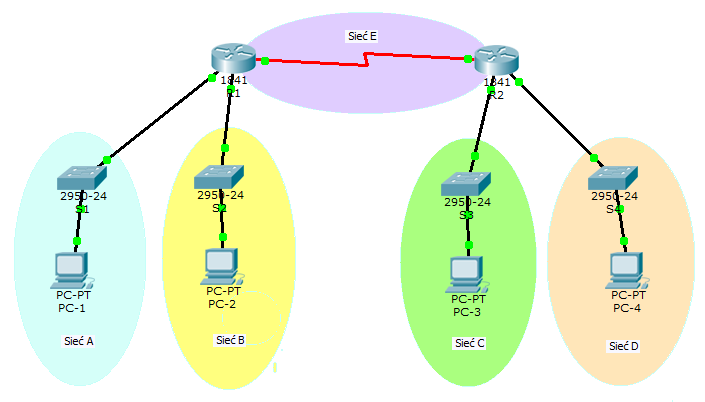
\includegraphics[width=11cm]{schemat}
\end{center}

\section{Zagadnienia}
% packet tracer, router, switch 
{\bf Packet Tracer} - symulator sieciowy firmy Cisco służący do budowania projektów sieci z wykorzystaniem ich urządzeń.\\
{\bf Sieć komputerowa} – zbiór komputerów i innych urządzeń połączonych z sobą kanałami
komunikacyjnymi oraz oprogramowanie wykorzystywane w tej sieci. Umożliwia ona wzajemne
przekazywanie informacji oraz udostępnianie zasobów własnych między podłączonymi do niej
urządzeniami. \\
{\bf Switch} - urządzenie sieciowe pozwalające na przyłączenie większej ilości hostów do sieci, switch sprawdza adresata pakietu i dostarcza go w odpowiednie miejsce.\\
{\bf Router} - urządzenie sieciowe przekazujące pakiety między dwoma segmentami sieci.\\
{\bf Routing} - wyznaczanie trasy i wysłanie nią pakietu danych w sieci komputerowej. \\

\section{Opis zadań}

1. Wybór urządzeń, dodanie portu serialowego do routerów,

połączenie według schematu \\
2. Ustawienie adresów dla wszystkich interfejsów na routerach \\
3. Ustawienie serwerów DHCP sieci: A, B, C i D \\
4. Ustawienie routingu statycznego na obydwu routerach \\

\begin{center}
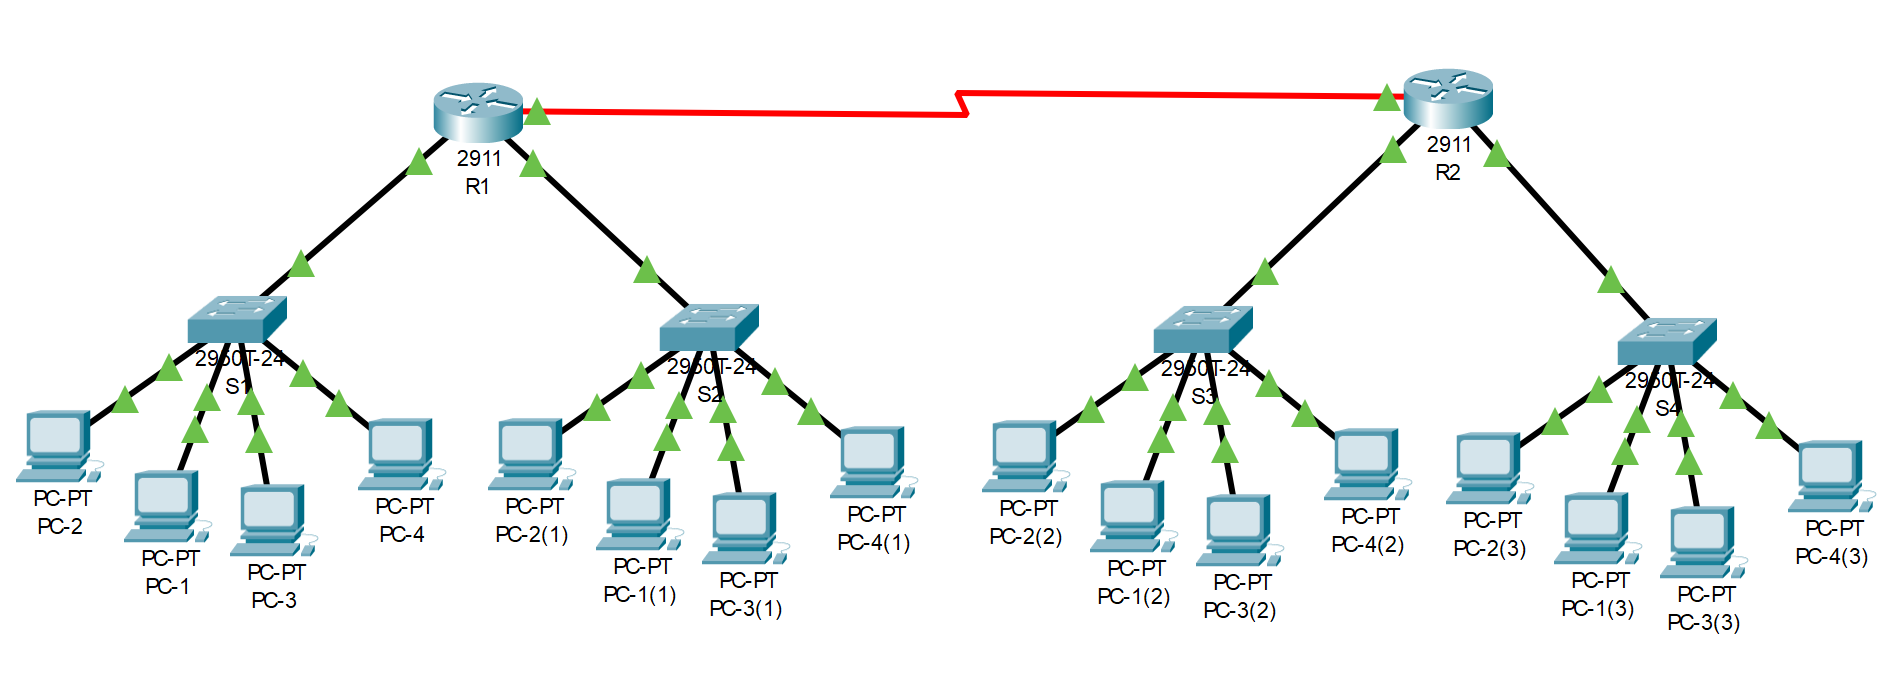
\includegraphics[width=14cm]{schematPacket}
\end{center}

\newpage
\section{Literatura}
Wikipedia:

\url{https://pl.wikipedia.org/wiki/Trasowanie_(telekomunikacja)}

\url{https://pl.wikipedia.org/wiki/Sieć_komputerowa}

\end{document}
